\documentclass[tikz]{standalone}
\usepackage{tikz}

\begin{document}    
	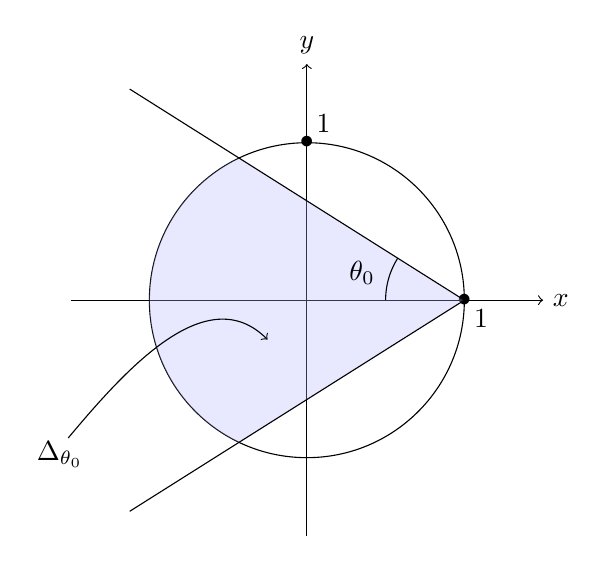
\begin{tikzpicture}
		\draw[->] (-3, 0) -- (3, 0) node[right] {$x$};
		\draw[->] (0, -3) -- (0, 3) node[above] {$y$};
		\draw(0,2) node {$\bullet$};
		\draw(0,2) node[above right]{$1$};
		\draw(2,0) node {$\bullet$};
		\draw(2,0) node[below right]{$1$};
		\draw (0,0) circle (2);
		\coordinate (A) at (130:3.5);
		\coordinate (B) at (230:3.5);
		\coordinate (C) at (2,0);
		\begin{scope}
			\path[clip] circle (2);
			\path[clip] (A) -- (B) -- (C) -- cycle;
			\draw [transparent, fill=blue!30, fill opacity=0.3] (C) circle (9);
		\end{scope}
		\begin{scope}
			\path[clip] (A) -- (180:3.5) -- (C) -- cycle;
			\draw (C) circle (1);
		\end{scope}
		\draw(0.7,0.35) node {$\theta_0$};
		\draw (C) -- (A);
		\draw (C) -- (B);
		\coordinate (S) at (210:3.5);
		\coordinate (E) at (-0.5,-0.5);
		\draw [->] (S) to [out=50] (E);
		\draw (212:3.7) node {$\Delta_{\theta_0}$};
	\end{tikzpicture}
\end{document}